\documentclass{beamer}
%
% Choose how your presentation looks.
%
% For more themes, color themes and font themes, see:
% http://deic.uab.es/~iblanes/beamer_gallery/index_by_theme.html
%
\mode<presentation>
{
  \usetheme{default}      % or try Darmstadt, Madrid, Warsaw, ...
  \usecolortheme{default} % or try albatross, beaver, crane, ...
  \usefonttheme{default}  % or try serif, structurebold, ...
  \setbeamertemplate{navigation symbols}{}
  \setbeamertemplate{caption}[numbered]
  \overfullrule  
} 

\usepackage[english]{babel}
\usepackage[utf8x]{inputenc}
%\usepackage{pdftex}
\usepackage{graphicx}
%\usepackage{wrapfig}  -- used for wrapping text around an image
\usepackage{lipsum}  % used to generate dummy text e.g. \lipsum[2-4]
\usepackage{multicol}

\title[Your Short Title]{Lewis Gaylon Hansen Letters}
\author{Steven L. Hansen}
\date{February 2017}


\begin{document}

\begin{frame}
  \titlepage
\end{frame}

% define Table of Contents
%
%   \section{<heading>}             -> to provide main sections 
%   \subsection{<sub-heading>}      -> to provide sub-sections
%
\begin{frame}{Table of Contents}
  \tableofcontents
\end{frame}

\section{Introduction}

\begin{frame}{Introduction}
%\lipsum[2-4]
some text
\end{frame}

\section{1961}
\subsection{College - Letter 1}
\begin{figure}
  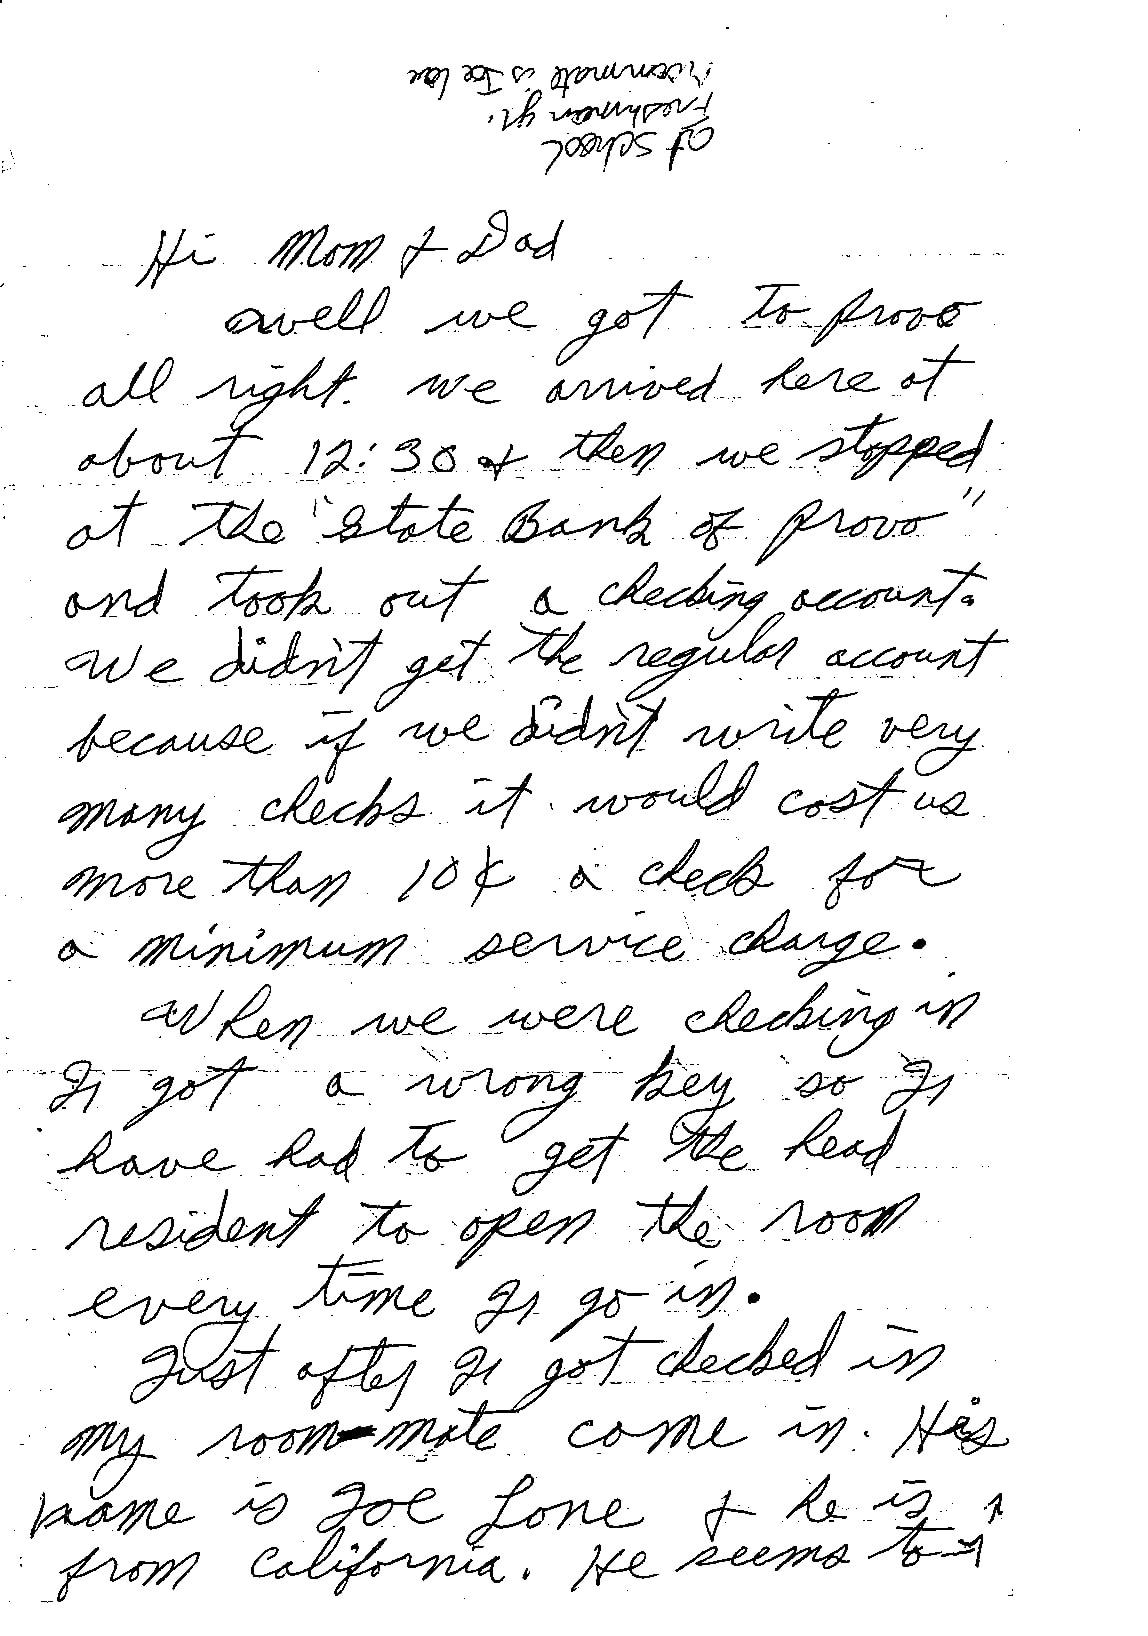
\includegraphics[scale=0.5]{1961/1961_letter_1_1.jpg}
\end{figure}

\begin{frame}{College - Letter 1}
\begin{multicols}{2}
%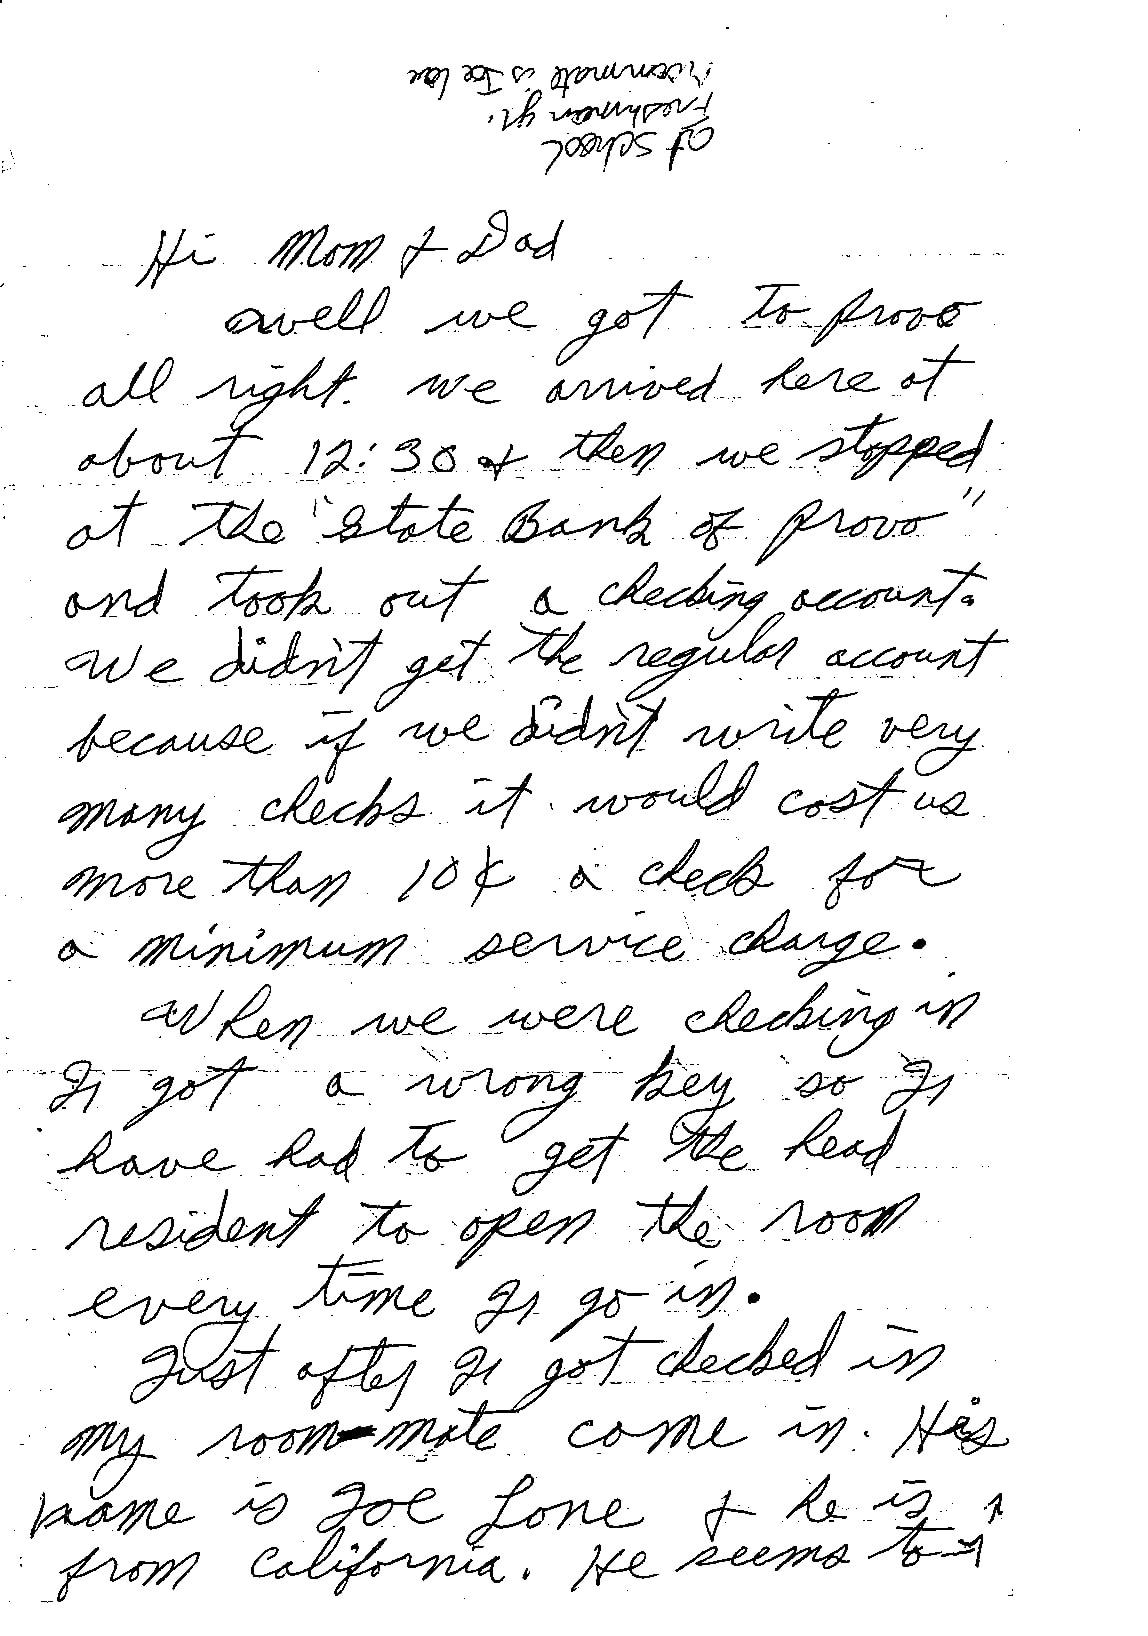
\includegraphics[width=0.50\textwidth]{1961/1961_letter_1_1.jpg}
%\lipsum[1]


second column text
%\lipsum[1]
\end{multicols}

\end{frame}



\subsection{College - Letter 2}
\begin{frame}{College - Letter 2
%\begin{multicols}{2}
%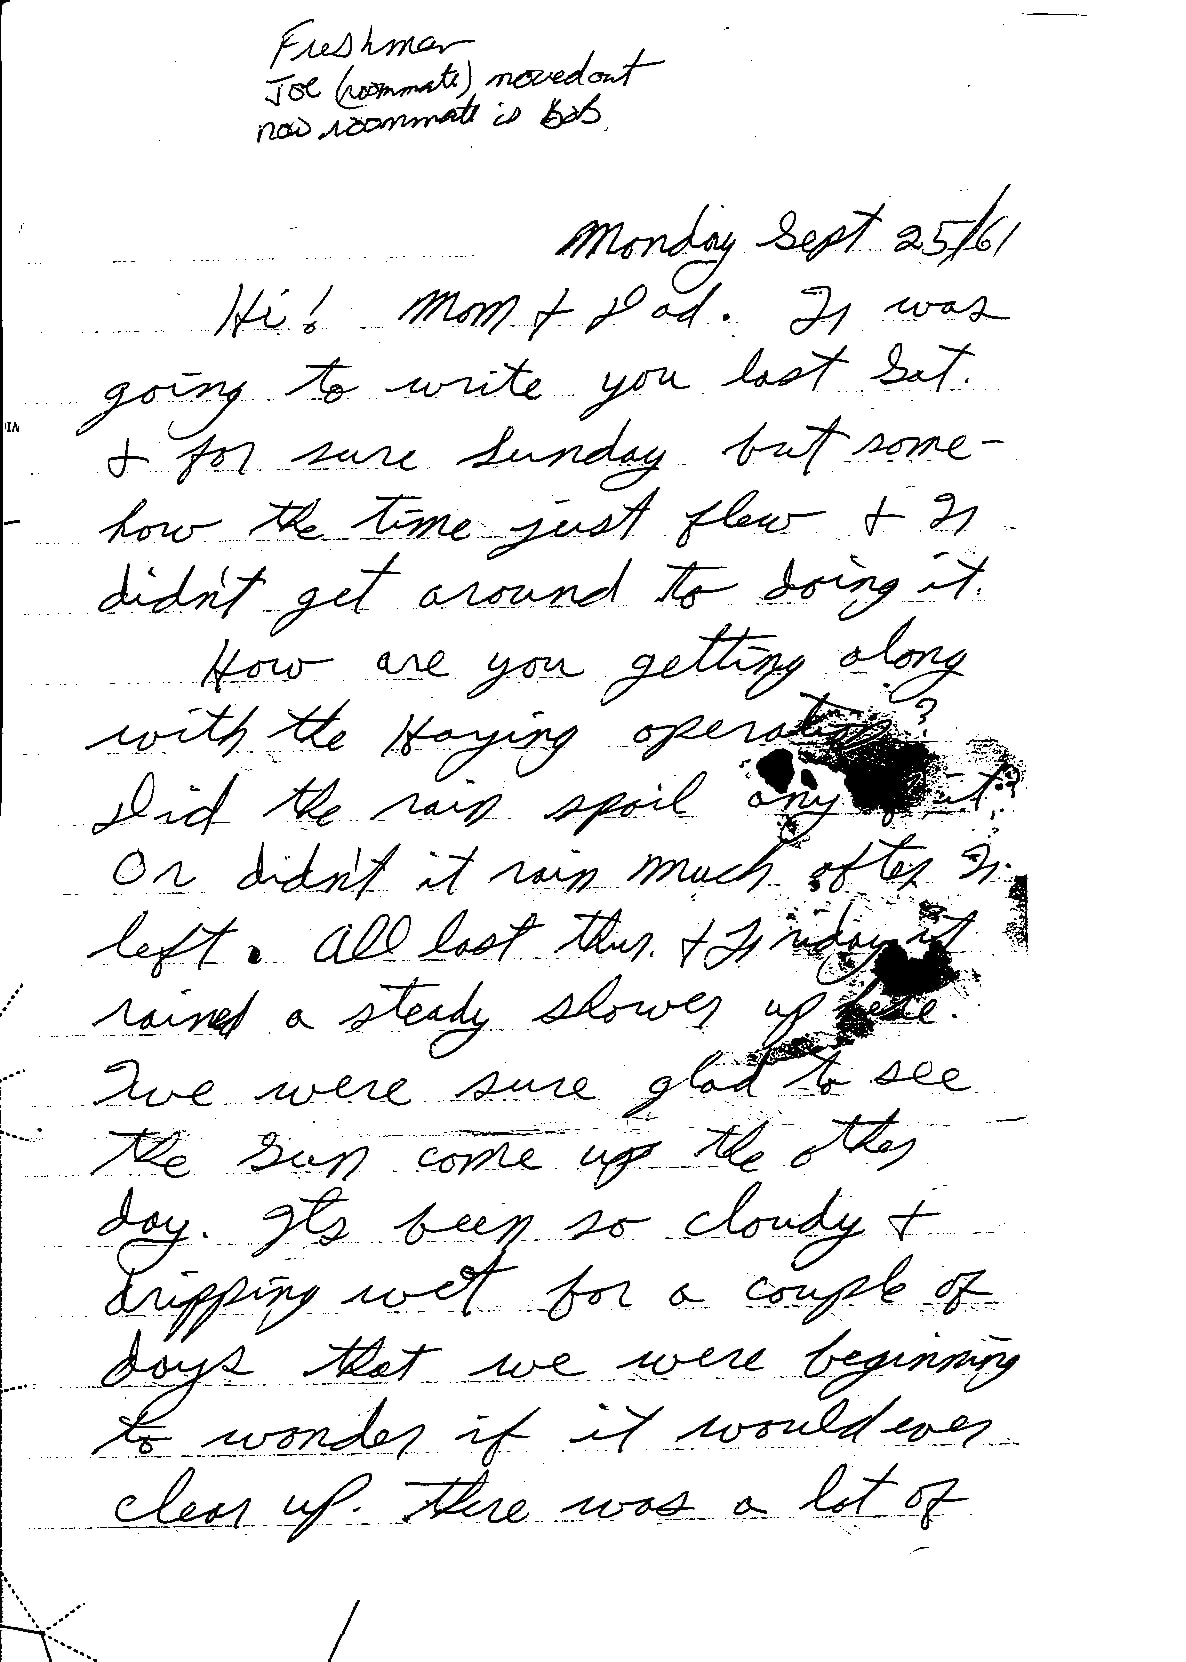
\includegraphics[width=\linewidth]{1961/1961_letter_2_0000.jpg}
%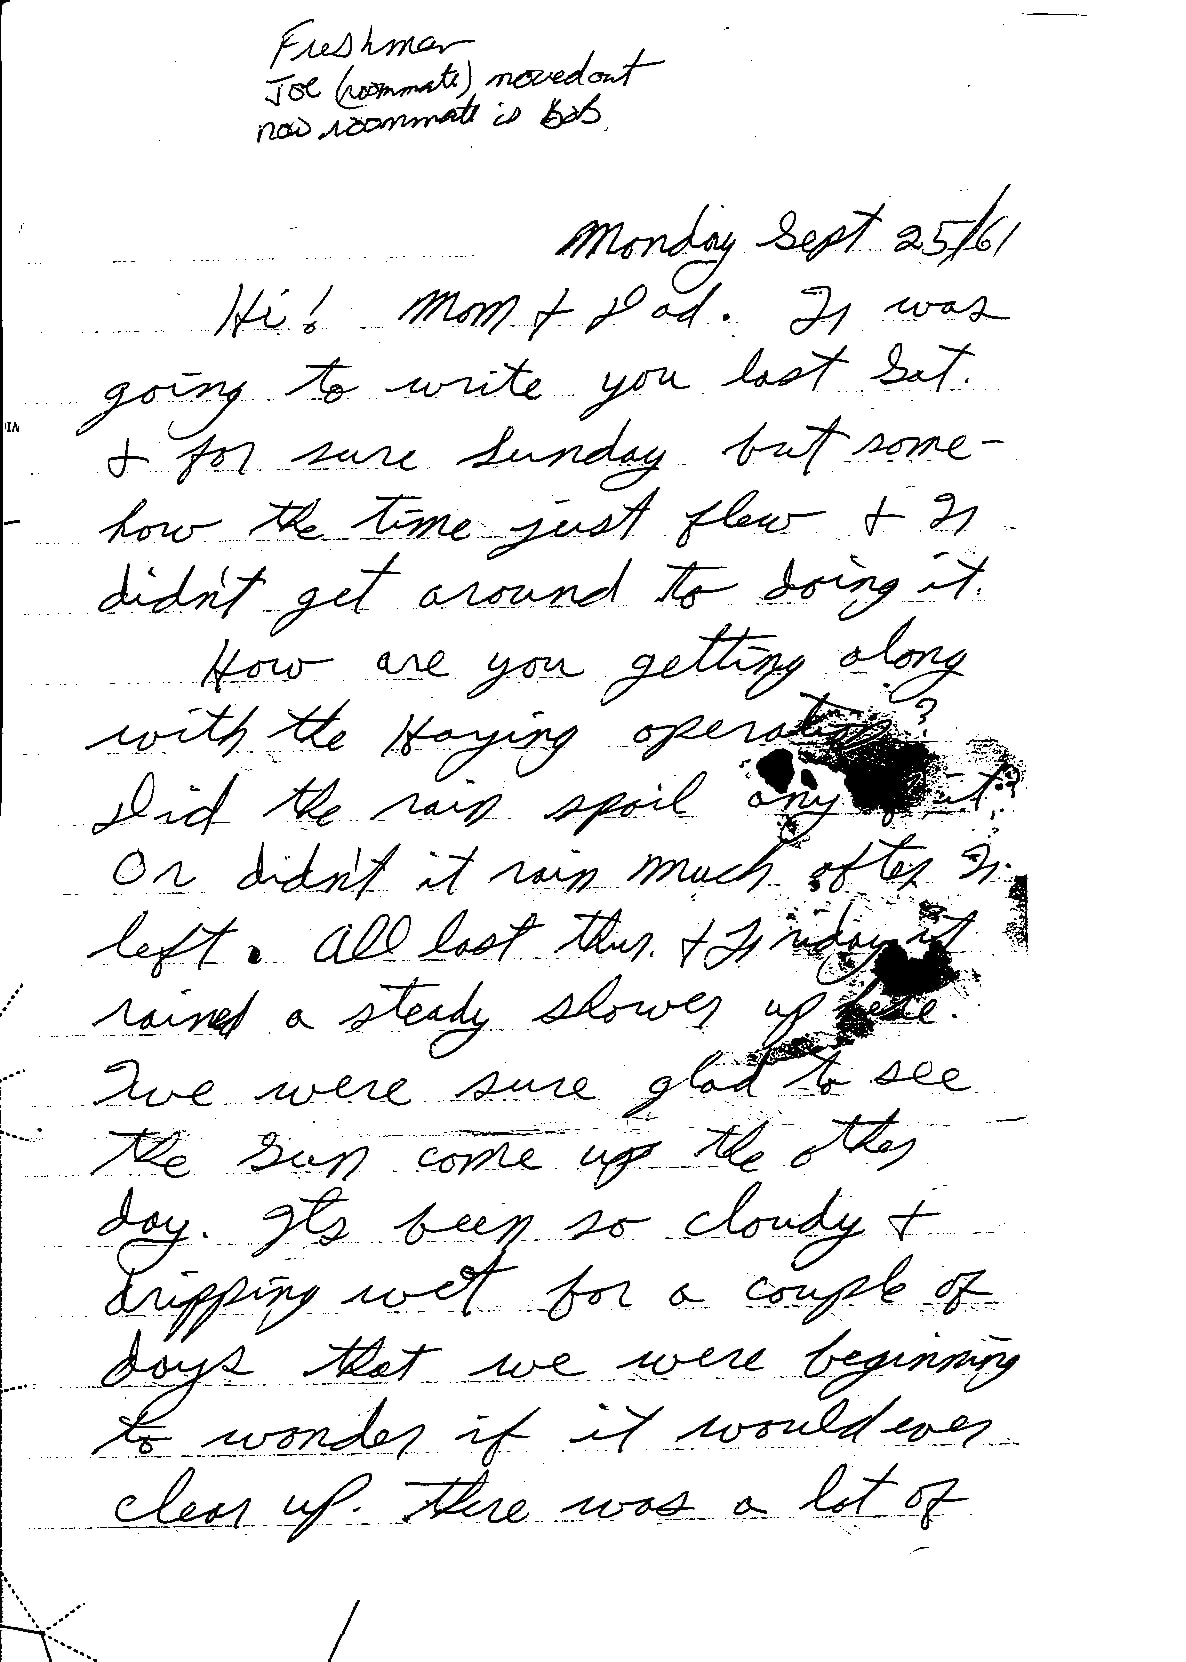
\includegraphics[width=0.50\textwidth]{1961/1961_letter_2_0000.jpg}



%\lipsum[1]
%\end{multicols}

\end{frame}
\end{document}
